\documentclass{article}

\usepackage{graphicx}
\usepackage{physics}
\usepackage{subcaption}
\usepackage{hyperref}

\usepackage[left=2.5cm, right=2.5cm, top=2.5cm, bottom=2.5cm]{geometry}
\setlength{\parindent}{0em}
\setlength{\parskip}{0.8em}

\usepackage{caption}
\captionsetup{width=.9\textwidth}

\usepackage[version=4]{mhchem}
\usepackage{siunitx}



\title{Exercise 3, TFY4235 Computational physics}
\author{Martin Johnsrud}
\vspace{-8ex}
\date{}


\begin{document}
    \maketitle
    \section*{Introduction}
        This paper documents the implementation and results of the simulation as given in \cite{exercise}. By using a finite difference scheme, the process of absorption of \ce{CO2} by the global ocean in the form of dissolved inorganic carbon (DIC). A simplified model of the physics is used, where both the atmospheric and oceanic concentration of carbon is constant at a given height, meaning there is in effect only one spatial dimension. The method is tested against known solutions, and the convergence is monitored. It is then used to extract results of how the ocean absorbs carbon, and at what rate.


    \section*{Theory and implementation}
    The implementation of the simulation largely follows \cite{exercise}, as laid out in the appendix. This section describes the particular choices made, and in a notation consistent with the code. The diffusion equation can be written as
    \begin{equation*}
        \Delta t \pdv{t} C(z, t) = \Delta t \left(K(z) \pdv[2]{z} + \dv{K(z)}{z}\pdv{z}\right) C(z, t) = \mathcal{D} C(z, t).
    \end{equation*}
    $\mathcal{D}$ is thus a linear operator which can be approximated by a discretization. With the scheme as descirbed in \cite{exercise}, and including the boundary condition this gives   
    \begin{equation*}
        \Delta t \pdv{t} C_n(t) = \mathcal{D}_{nm} C_n(t) + S_n(t),
    \end{equation*}
    where summation over repeated indices are implied, and
    \begin{align*}
        \mathcal{D} &=
        \begin{pmatrix}
            -4\alpha K_0 - 2\Gamma & 4\alpha K_0 & \dots & 0 & 0 \\
            \vdots & \ddots & \ddots & 0 & 0\\
            0 & -\frac{\alpha}{2} K_i' + 2\alpha K_i & -4 \alpha K_i & \frac{\alpha}{2}K_i' + 2\alpha K_i & 0 \\
            0 & 0 & \ddots & \ddots & \vdots\\
            0 & 0 & \dots & 4\alpha K_N & -4\alpha K_N
        \end{pmatrix}, \quad \alpha = \frac{\Delta t}{2 \Delta z^2 },\\
        S(t) & =  
        \begin{pmatrix}
            2\Gamma C_\mathrm{eq}(t) &0&\dots&0
        \end{pmatrix}^T \quad 
    \Gamma = 2 \frac{\alpha k_w \Delta z}{K_0} \left(K_0 - \frac{1}{2}(-\frac{3}{2} K_0 + 2K_1 - \frac{1}{2}K_2)\right), \quad
      K_n' = K_{n+1} - K_{n-1}.
    \end{align*}
    Using the Cranck-Nichelson scheme to discretize the time part yields
    \begin{equation*}
        C_n^{i+1}  = C_n^i + \frac{1}{2} (\mathcal{D}_{nm} C_m^i + S_n^i) + \frac{1}{2} (\mathcal{D}_{nm} C_m^{i+1} + S_n^{i+1}),
    \end{equation*}
    so the equation to be solved to get the next timestep is
    \begin{align*}
        A_{nm} C_{m}^{i+1} = V_n^i, \quad V_n^i = \left(\delta_{nm} + \frac{1}{2} \mathcal{D}_{nm}\right) C_m^i + \frac{1}{2}(S_n^i + S_n^{i+1}), \quad 
        A_{mn} = \left(\delta_{nm} - \frac{1}{2} \mathcal{D}_{nm}\right).
    \end{align*}
    
    The implementation of this system of equation uses SciPy's sparse matrix library. After creating sparse realizations of $A$, SciPy's \verb|splu| is used to generate the LU decomposition \verb|LU| of $A$. This is an object with methods such as \verb|.solve()|, which utilizes the LU decomposition. The wrapper \verb|simulate| then loops over $N_t-1$ steps, using \verb|solve(V) = lambda V: LU.solve(V)|, where \verb|V| is as given above.

    The results of the simulation of $C$ is kept in a NumPy array. However, it is not necessary to keep all steps made in time. \verb|simulate| can be passed a integer argument \verb|save|, the number of time steps to be kept in the array. This entails that $N_t-1$ is divisible by $\mathrm{save}-1$, which is checked by an \verb|assert| statement.

    To check convergence of the method, both in time and space, a way of measuring error is needed. In this project, relative root mean square (RMS) error is used. Given a concentration $C(z)$ and a reference $C_0(z)$ at a given time, sampled at a set of points $\{z_i\}_{i=1}^N \in [0, L]$, relative RMS error is given by
    \begin{equation*}
        \Delta_\mathrm{rms} = \sqrt{\frac{1}{N}\sum_i \left(\frac{C(z_i) - C_0(z_i)}{C_0(z_i)}\right)^2}.
    \end{equation*}
    When comparing concentrations with different values for $N_z$, as is necessary to find the convergence of the method in space, one must make sure that the points of comparison are the same for both $C$ and $C_0$. This is done by setting $N_z = 5\cdot 2^Na + 1$ for $C_0$, and $N_z = 2^n a + 1$. Here, $a$ and $N$ are integers, and $n$ is some integer less or equal to $N$. This ensures that the set of points $\{z_i\}_{i=1}^{2^na+1}$ that $C(z)$ is simulated on, $C_0(z)$ is as well, and they can be compared. This is implemented by \verb|get_rms| in \verb|utilities.py|, which takes a list of arrays and compare each with the last element. 


    \section*{Tests}
    Make sure the implementation gives good answers, it is compared to known solutions. The method used in this implementation has quadratic convergence, both in time and space. A convergence test was implemented for a simple test case, to check this. \autoref{convergence test} shows the result of this. 

    \begin{figure}
        \centering
        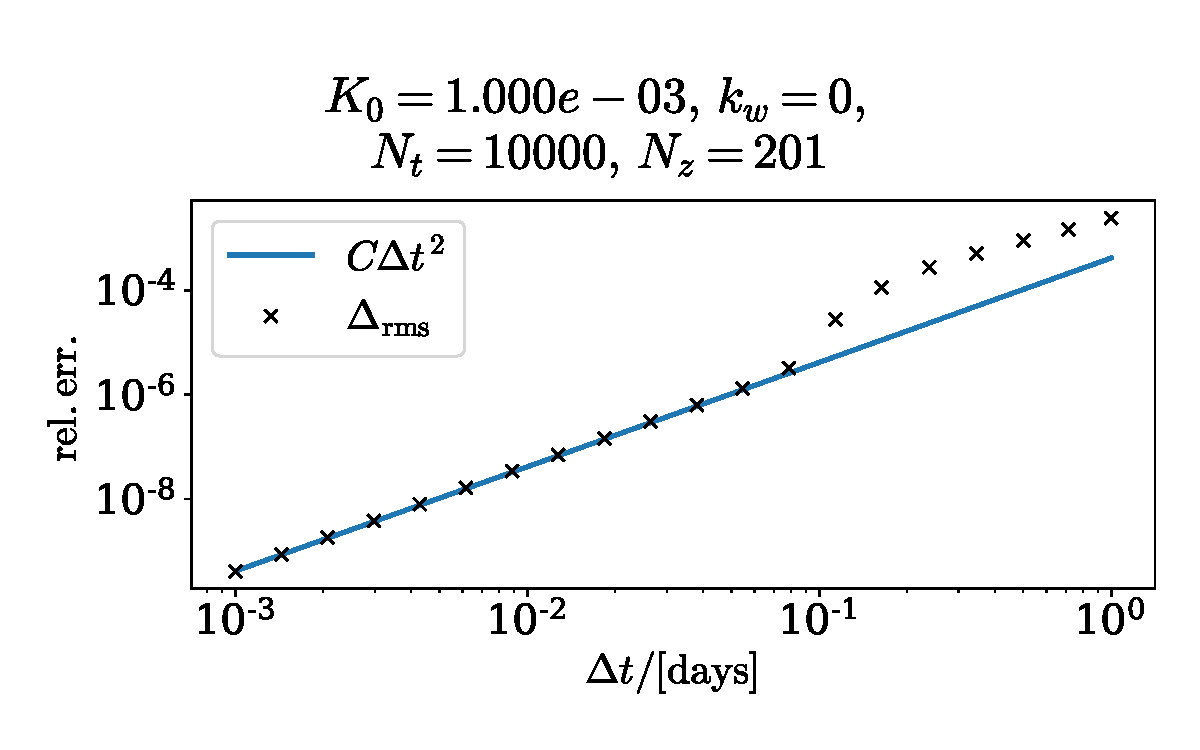
\includegraphics[width=.49\textwidth]{../plots/conv_test_t}
        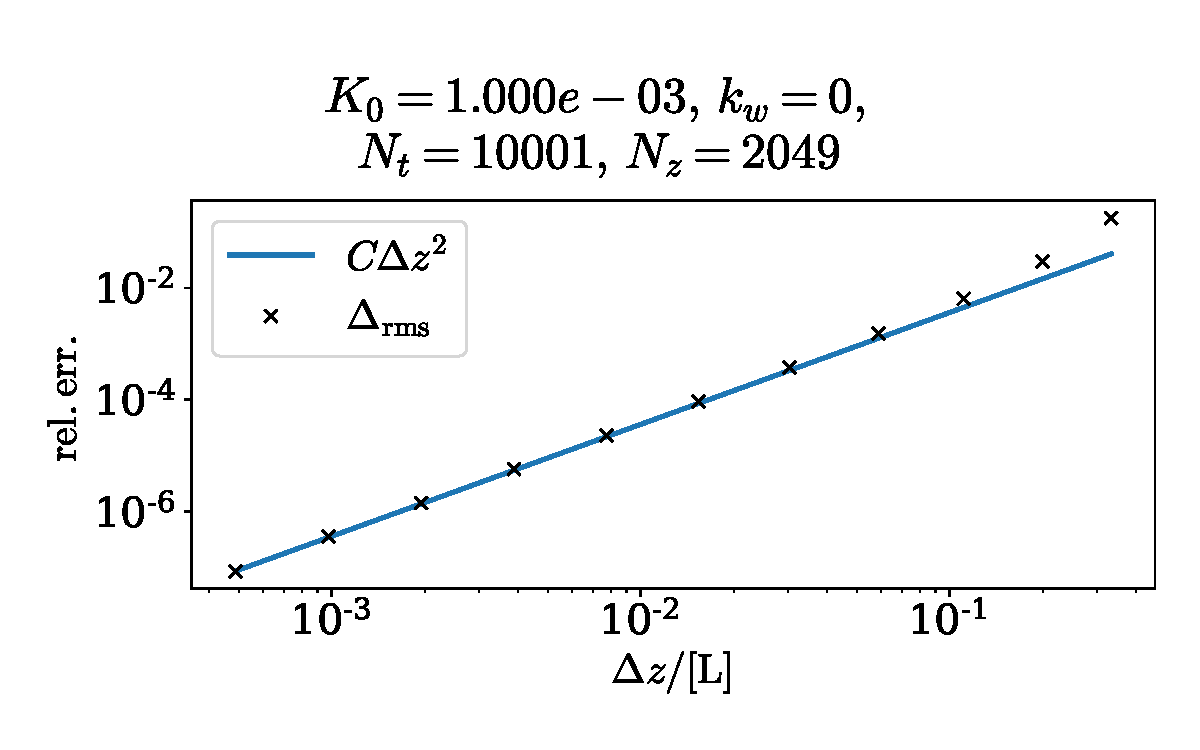
\includegraphics[width=.49\textwidth]{../plots/conv_test_z}
        \caption{Error, measured as the root mean square deviation from a reference value, after 1 day simulation of an Gaussian initial concentration.}
        \label{convergence test}
    \end{figure}

    A constant concentration of \ce{CO2} should remain constant, regardless of $K(z)$, as long as it is positive. This test is shown in \autoref{constant_cons}, with a both a constant $K(z)$, and a smooth step function between two values of $K$. For both, the constant initial concentration is close to unchanged, save for numerical errors.

    \begin{figure}
        \centering
        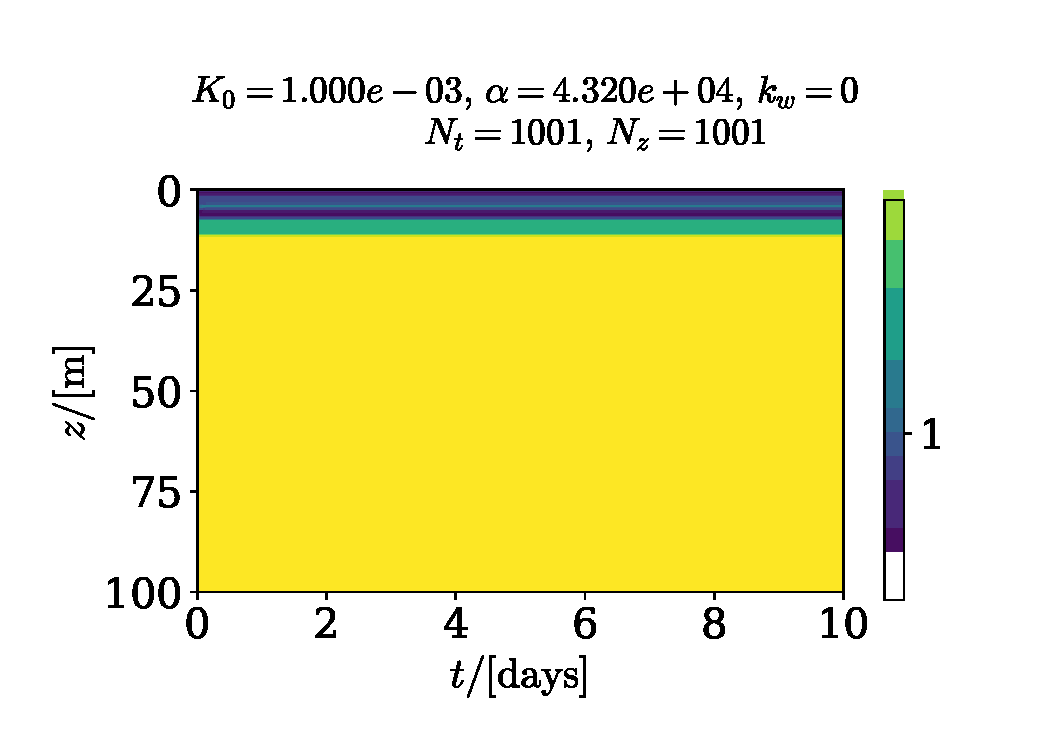
\includegraphics[width=.49\textwidth]{../plots/test1}
        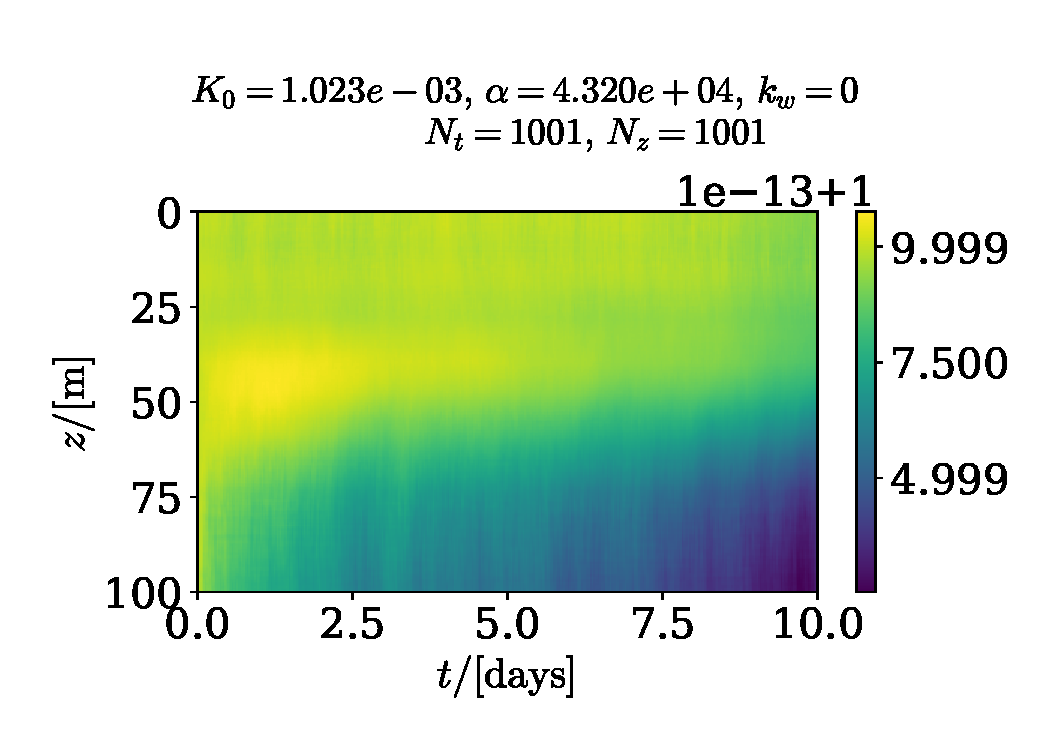
\includegraphics[width=.49\textwidth]{../plots/test1_varK}
        \caption{The time evolution of an constant concentration. The system on the left has a constant $K(z)$, while system of the right has an oscillatory $K$. The largest deviation of the system is of order $10^{-15}$ and $10^{-13}$, respectively.}
        \label{constant_cons}
    \end{figure}

    The systems should also, given $k_w=0$, conserve mass. To test this, a initial distribution of two Gaussian functions were evolved in time, with a non-constant diffusivity. The result is shown in \autoref{Consv mass}, where the mass is conserved to a good approximation.

    \begin{figure}
        \centering
        \includegraphics[width=.49\textwidth]{../plots/test2_c}
        \includegraphics[width=.45\textwidth]{../plots/test2_m}
        \caption{The evolution of a Gaussian distribution of \ce{CO2} is shown on the left. On the right, the relative change in mass as a function of time is plotted. }
        \label{Consv mass}
    \end{figure}

    A sharply peaked Gaussian package should have a variance that increases linearly with time, then approach a steady state. This is shown in \autoref{var}.

    \begin{figure}
        \centering
        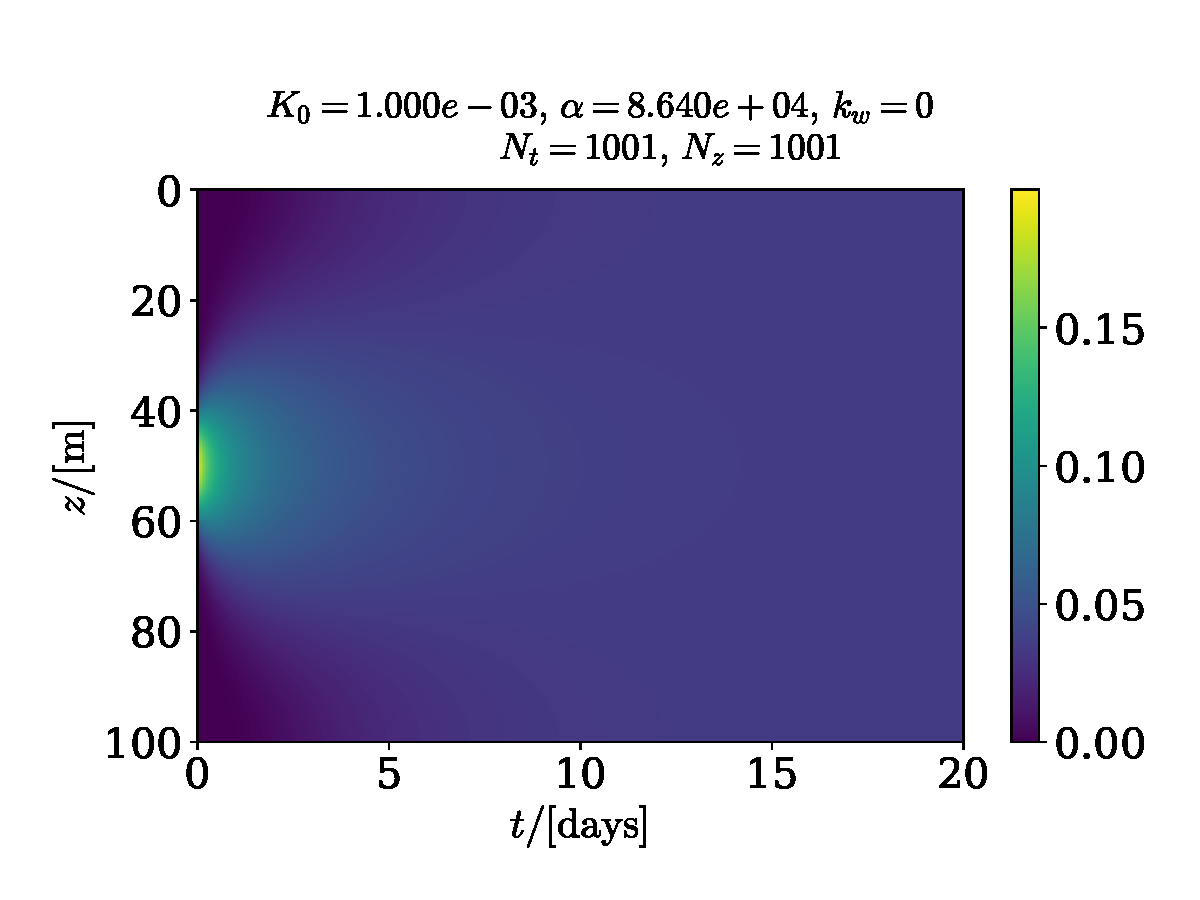
\includegraphics[width=.49\textwidth]{../plots/test3}
        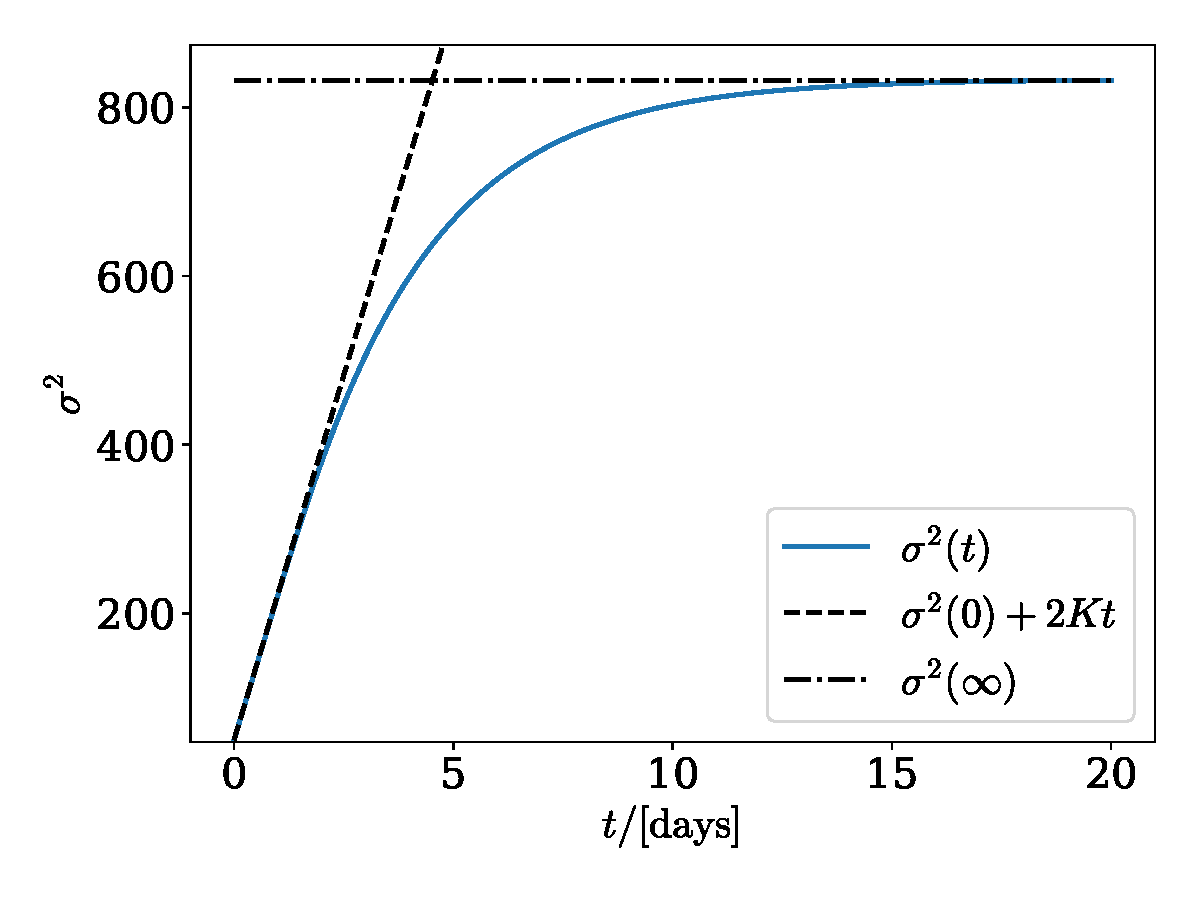
\includegraphics[width=.45\textwidth]{../plots/test3_var}
        \caption{A system with an initial Gaussain distribution is simulated. On the right, the variance as a function of time is shown. The increase is initially constant, but then approaches a steady state.}
        \label{var}
    \end{figure}

    \autoref{decay} shows the depletion of \ce{CO2} from the ocean, given a zero partial pressure in the atmosphere. For a small Biot number, this should follow a exponential decay, as this test shows.

    \begin{figure}
        \centering
        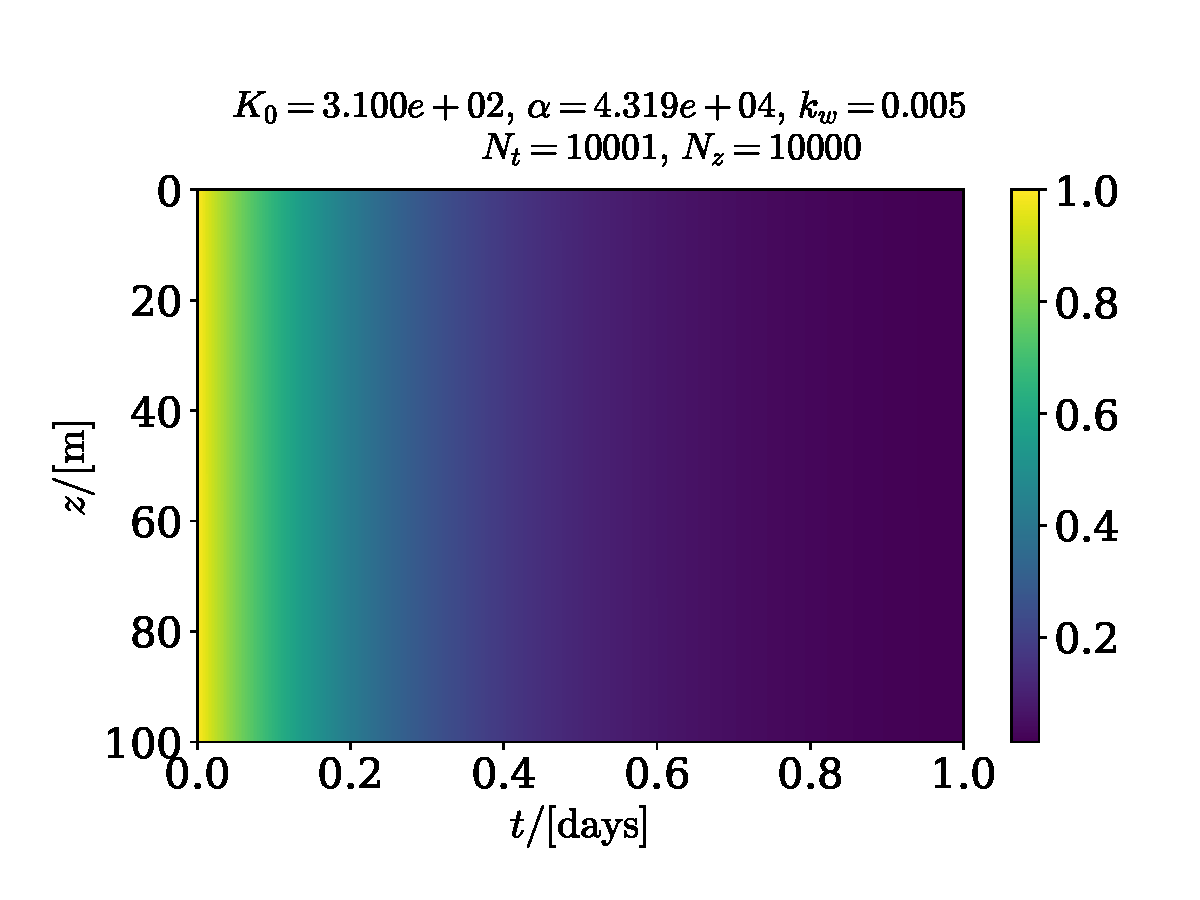
\includegraphics[width=.49\textwidth]{../plots/test4}
        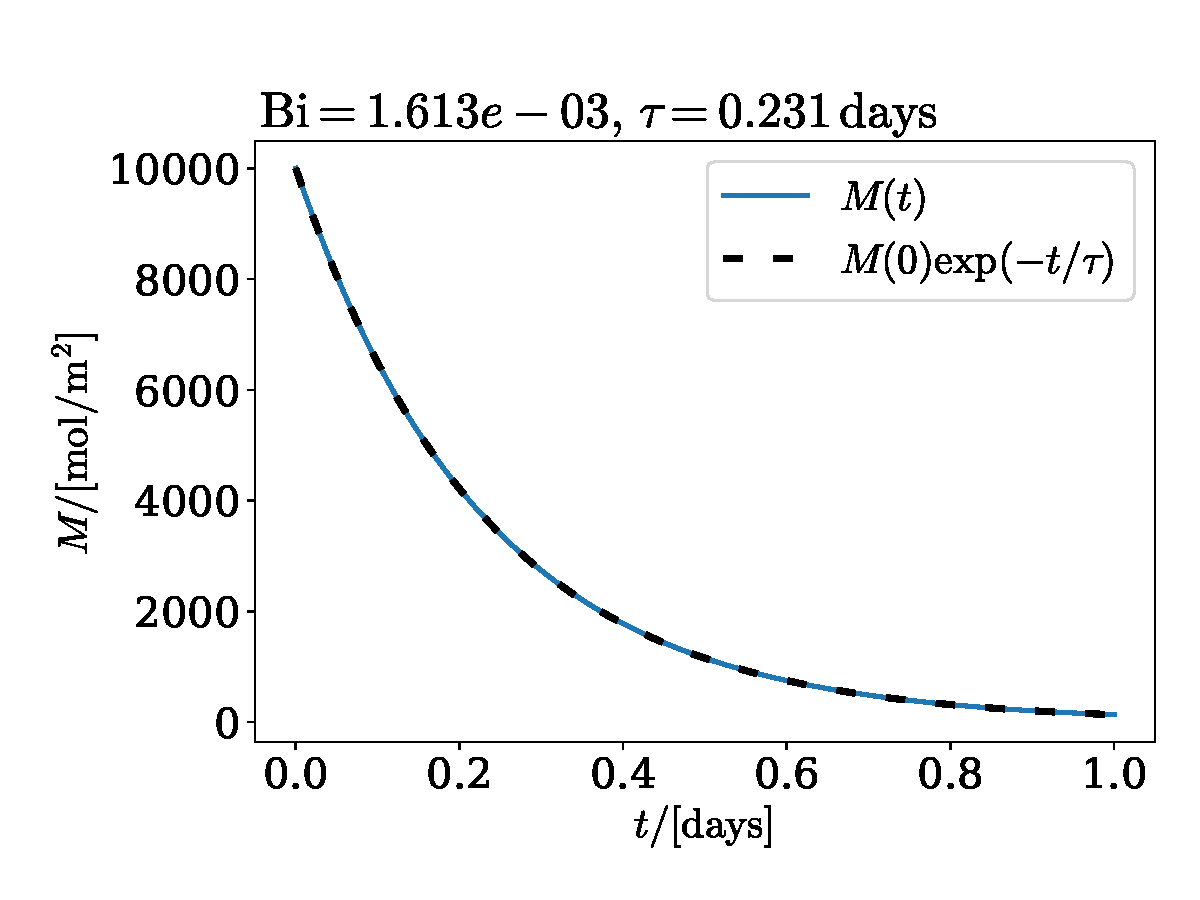
\includegraphics[width=.45\textwidth]{../plots/test4_decay}
        \caption{The slow removal of \ce{CO2} from the ocean, when the atmosphere contains a partial pressure of 0.}
        \label{decay}
    \end{figure}

    Lastly, \autoref{minmax} shows how the ocean reaches a equilibrium with the atmosphere, given a non-zero, positive mass-transfer coefficient $k_w$ and either constant or non-constant diffusivity.

    \begin{figure}
        \centering
        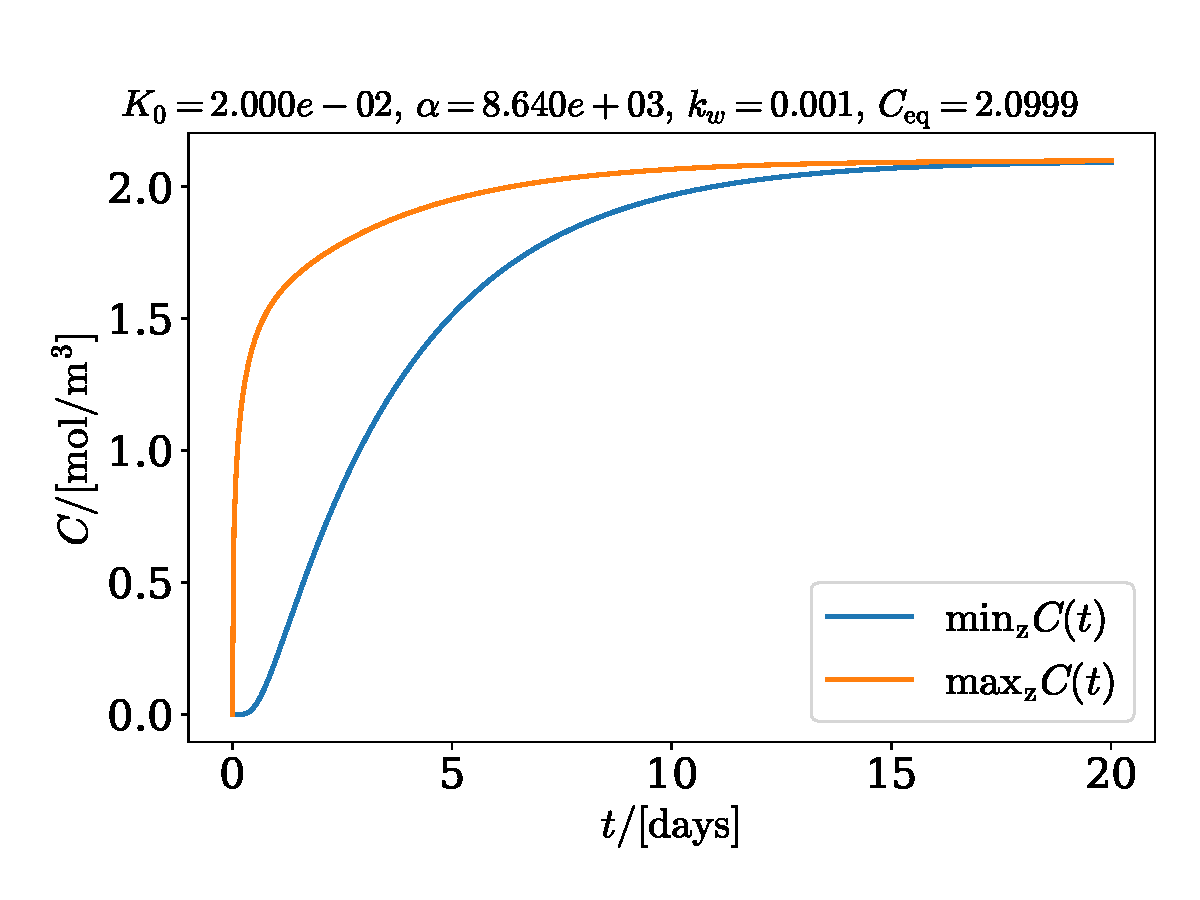
\includegraphics[width=.49\textwidth]{../plots/test5_minmax}
        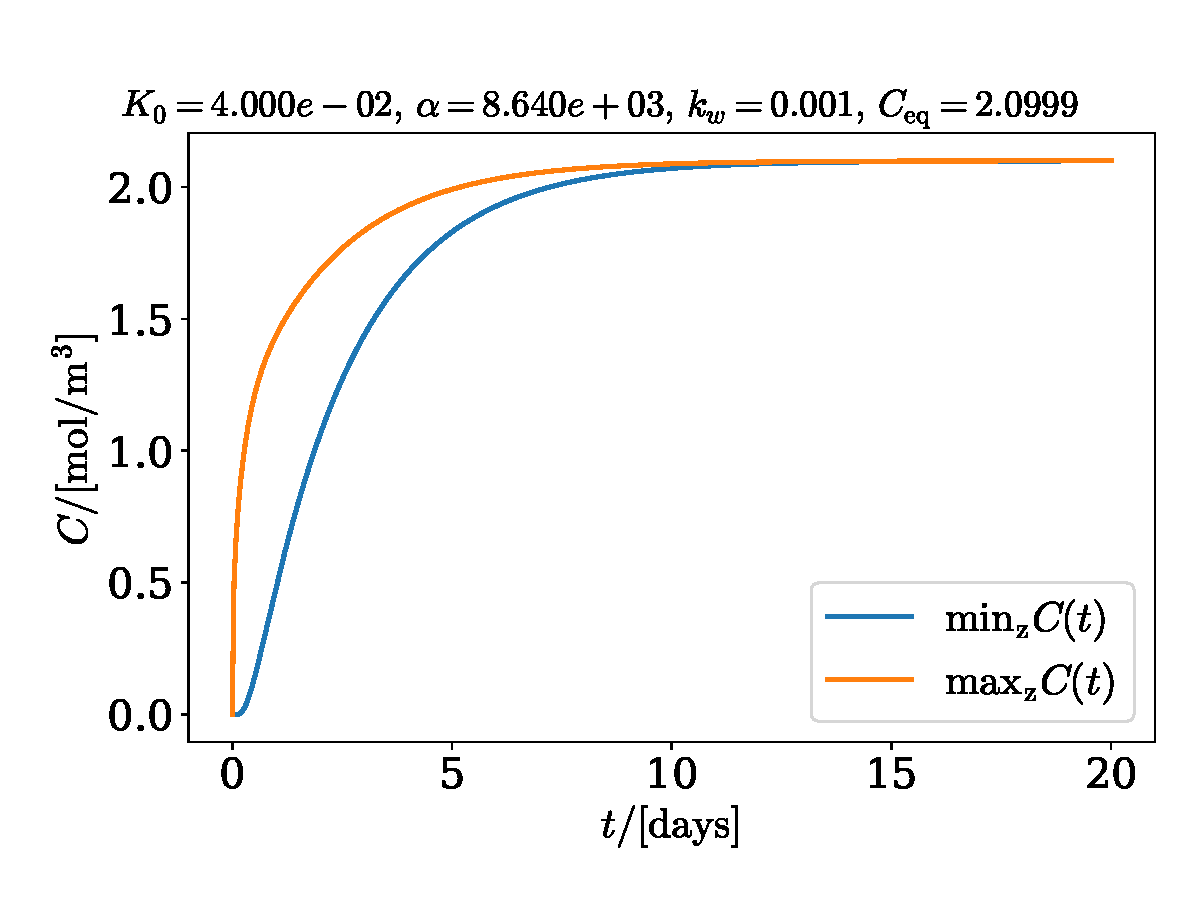
\includegraphics[width=.49\textwidth]{../plots/test5_varK_minmax}
        \caption{Equilibration of the ocean with a atmosphere with $C_\mathrm{eq}=0.5$. The figure on the left is a system with constant diffusivity, the left side has a oscillating but always positive diffusivity.}
        \label{minmax}
    \end{figure}

    \section*{Results}
    \subsubsection*{Shallow waters}
    To simulate the uptake of \ce{CO2} in shallow areas, $L=\SI{100}{m}$, diffusivity $K(z)$ is used as given in equation (11) in \cite{exercise}. \autoref{prob2 conv} illustrates the convergence of the simulation, which shows that the simulation still has quadratic convergence both in time and space. The convergence test are run for a time of $\SI{10}{days}$.

    \begin{figure}
        \centering
        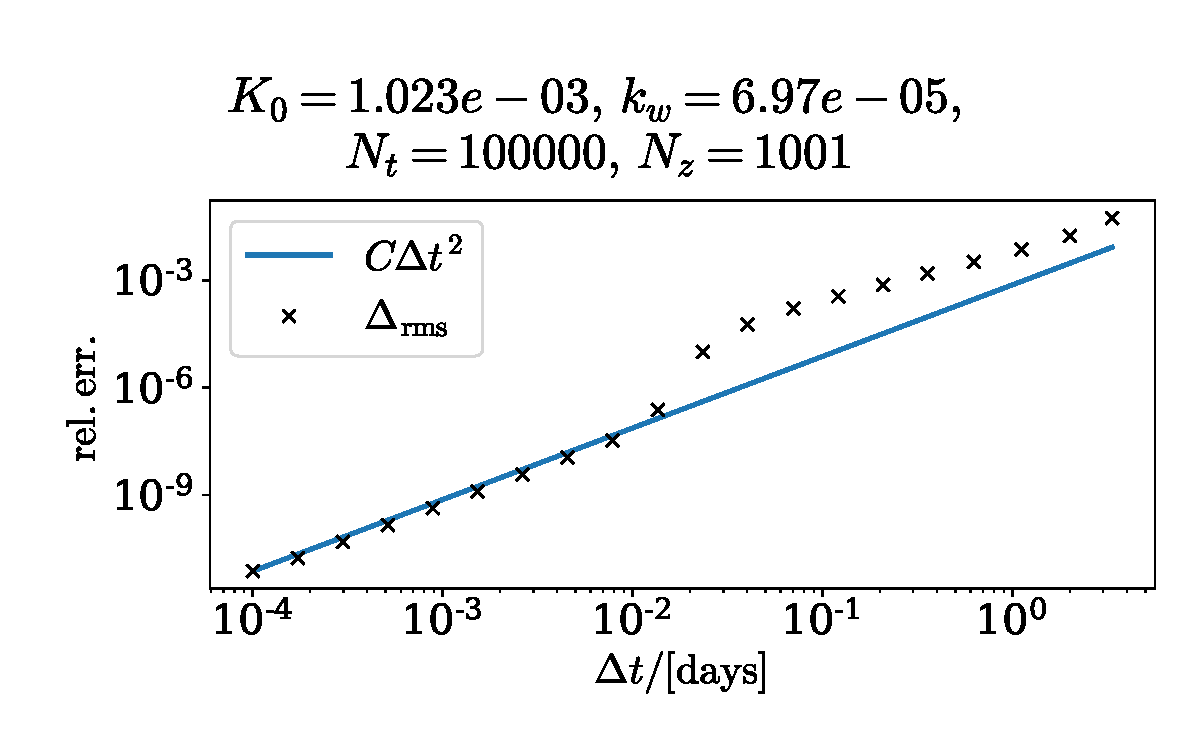
\includegraphics[width=.49\textwidth]{../plots/prob2_conv_test_t}
        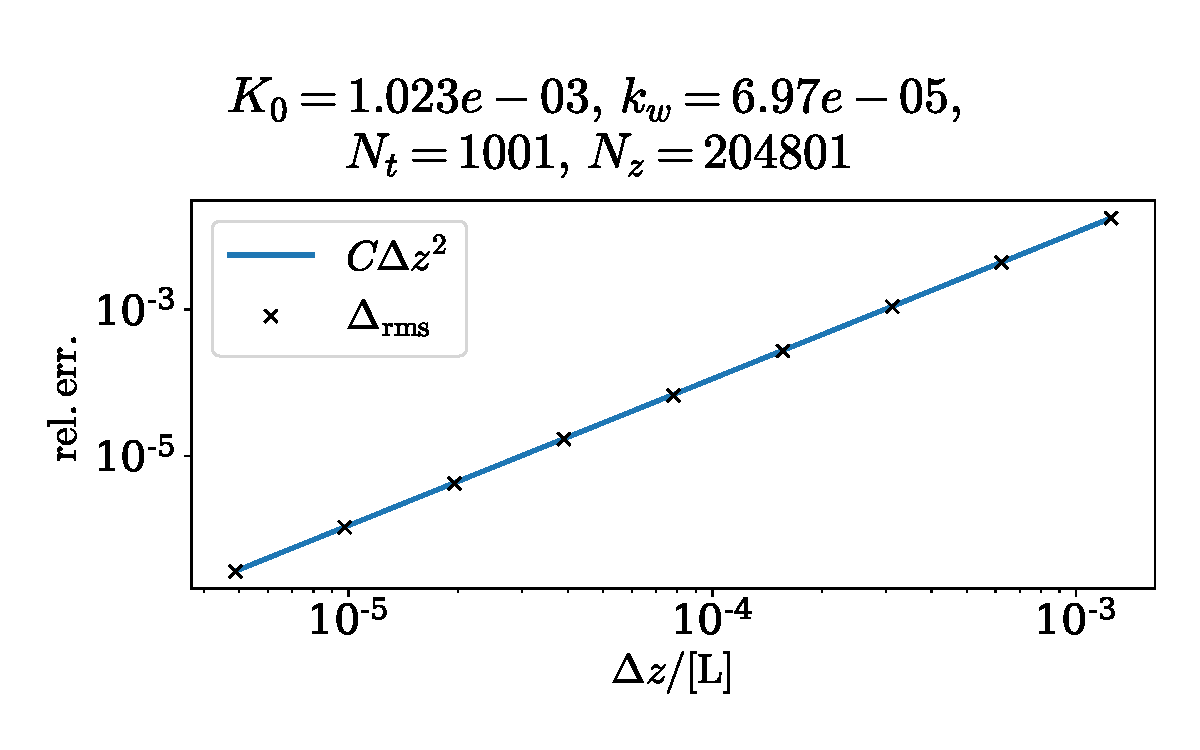
\includegraphics[width=.49\textwidth]{../plots/prob2_conv_test_z}
        \caption{Error, as a function of step length in both time and space.}
        \label{prob2 conv}
    \end{figure}

    The simulation is then run for 180 days, with $N_t = N_z = 10000$. This corresponds to $\Delta t = 180 / 10000 = 1.8 \cdot 10^{-2} \si{days}$, and $\Delta z = L/10000 = 10^{-4} L$. The results are shown in \autoref{prob2}, together with the form of the diffusivity, $K(z)$. \autoref{prob2 minmax} shows how the minimum and maximum concentration evolves as a function of time, together with some snap shots of the concentration as it evolves. The surface of the ocean, where wind dominates the diffusion, first absorbs the \ce{CO2}. The deeper parts of the ocean lacks behind some, as there low diffusivity around 40 meters are a bottle neck, but it does not take long before it penetrates down to the ocean floor.

    At 90 days, the ocean is nearly in equilibrium with the atmosphere, and at 180 it is so close as does not make a difference. This gives confidence to an assumption that the carbon in the ocean is in sync with the atmosphere.

    \begin{figure}
        \centering
        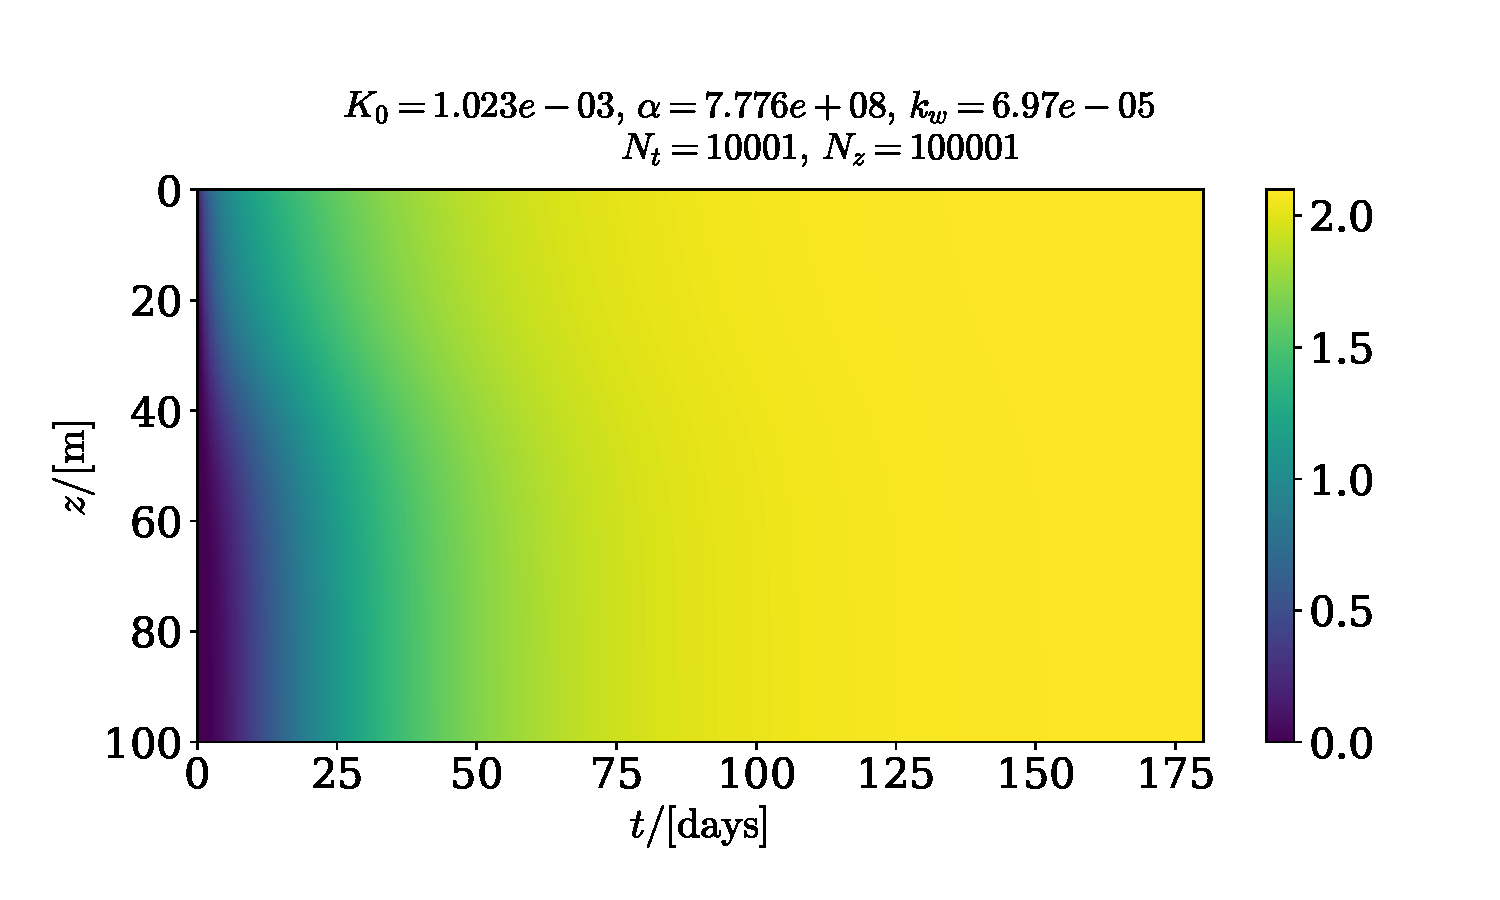
\includegraphics[width=.65\textwidth]{../plots/prob2}
        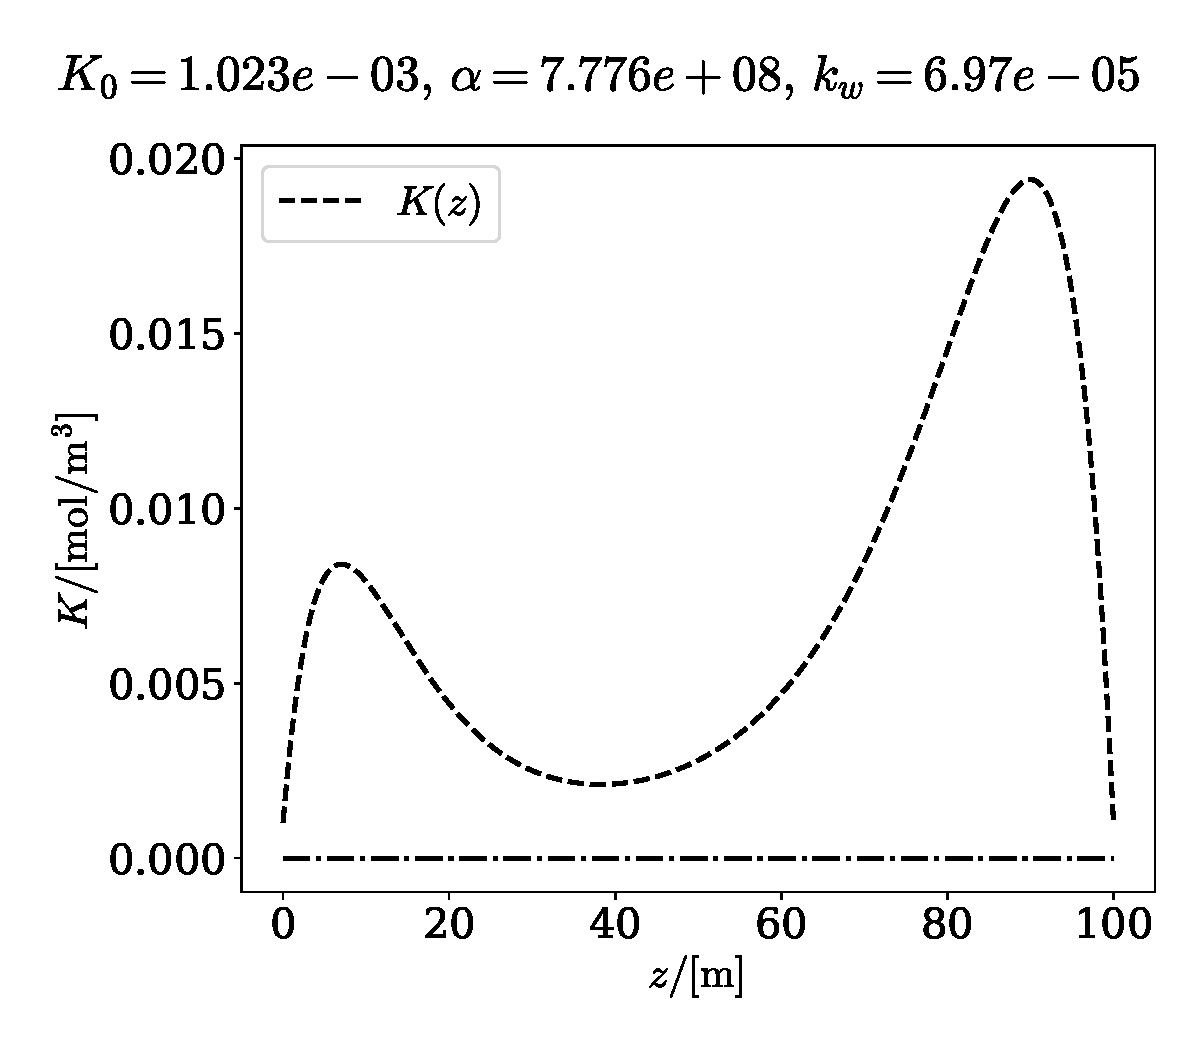
\includegraphics[width=.3\textwidth]{../plots/prob2_K}
        \caption{cap}
        \label{prob2}
    \end{figure}

    \begin{figure}
        \centering
        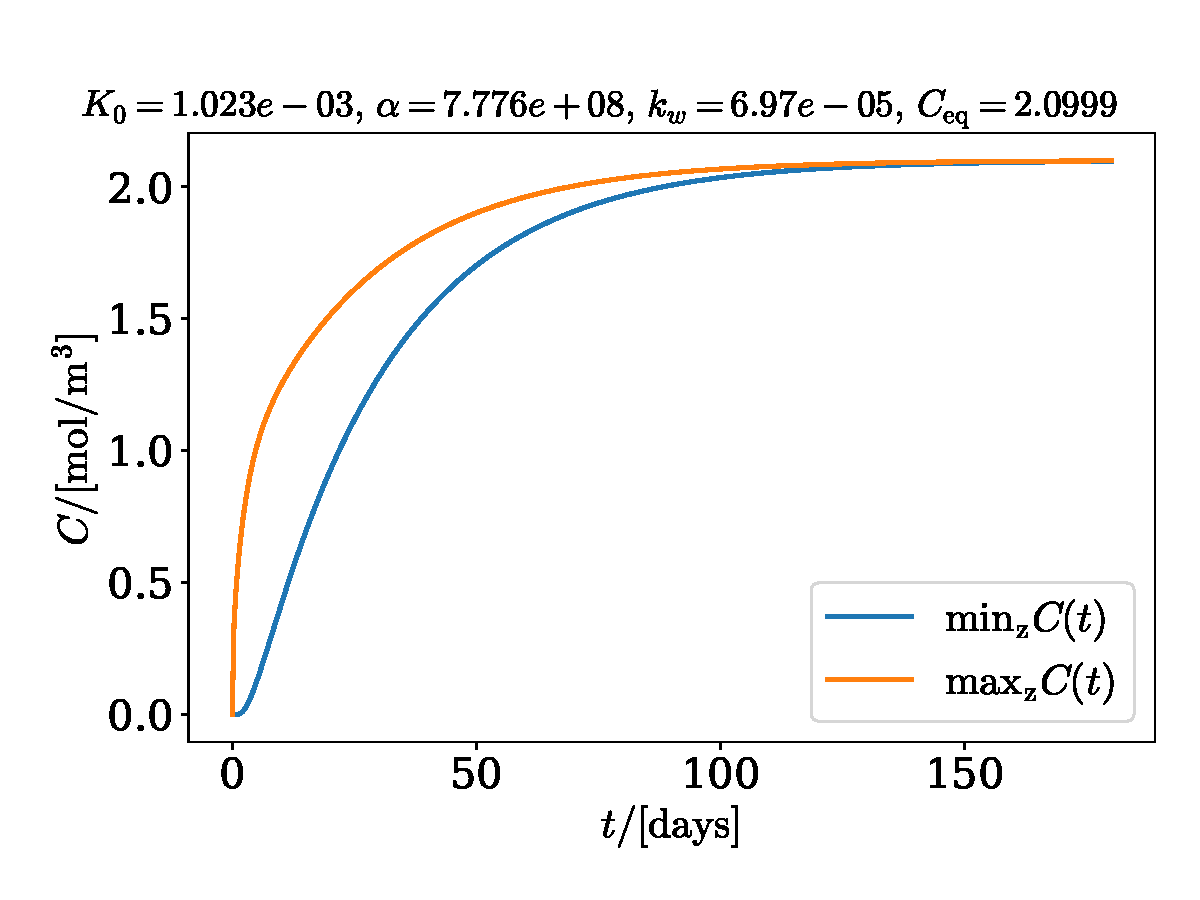
\includegraphics[width=.47\textwidth]{../plots/prob2_minmax}
        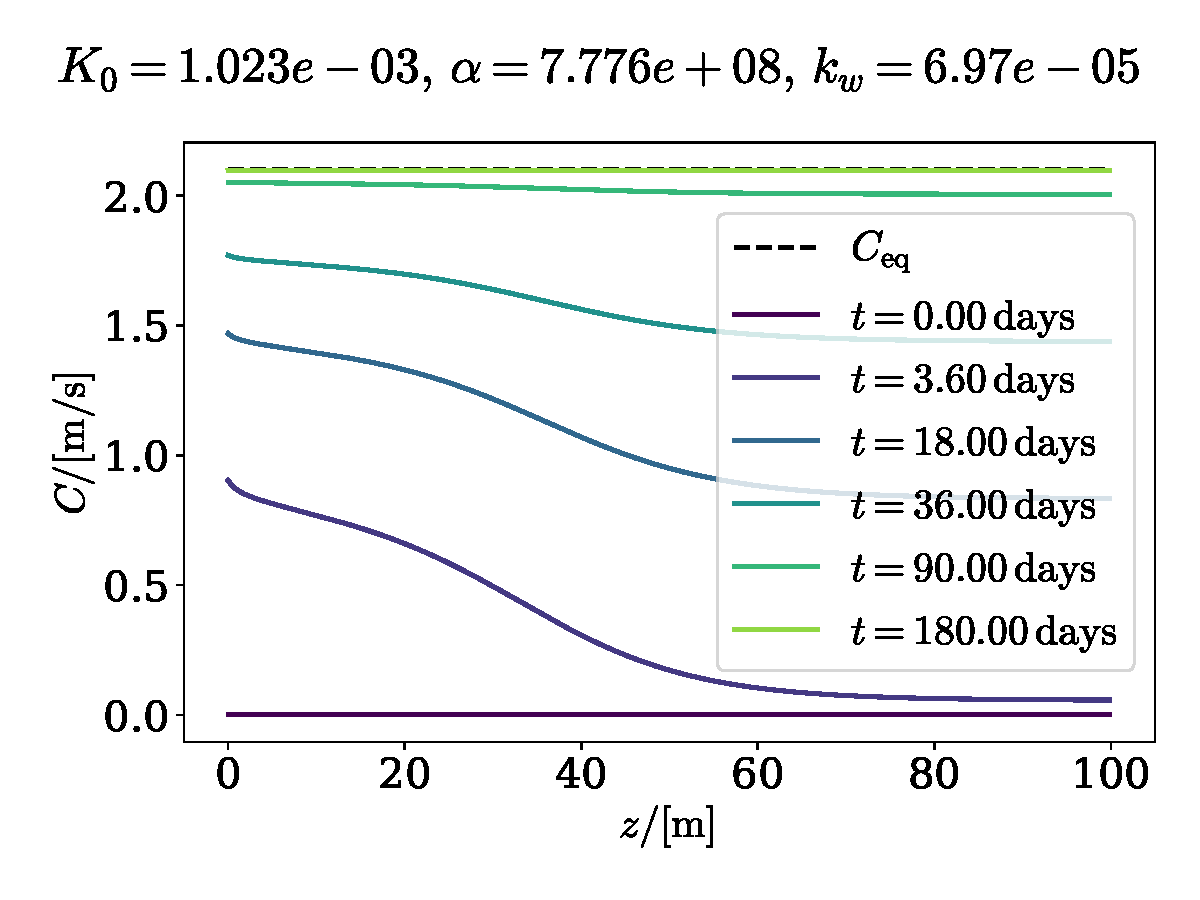
\includegraphics[width=.52\textwidth]{../plots/prob2_i}
        \caption{cap}
        \label{prob2 minmax}
    \end{figure}

    \subsubsection*{Deep waters}
    In this section, the ocean is modeled as $\SI{4000}{m}$ deep, and with a 2-layered diffusivity. This model is run for a longer time of several years, and therefore includes the increase in \ce{CO2} in the atmosphere. \autoref{prob3 conv} shows the convergence of the simulation, confirming the simulation still converges quadratically.

    \begin{figure}
        \centering
        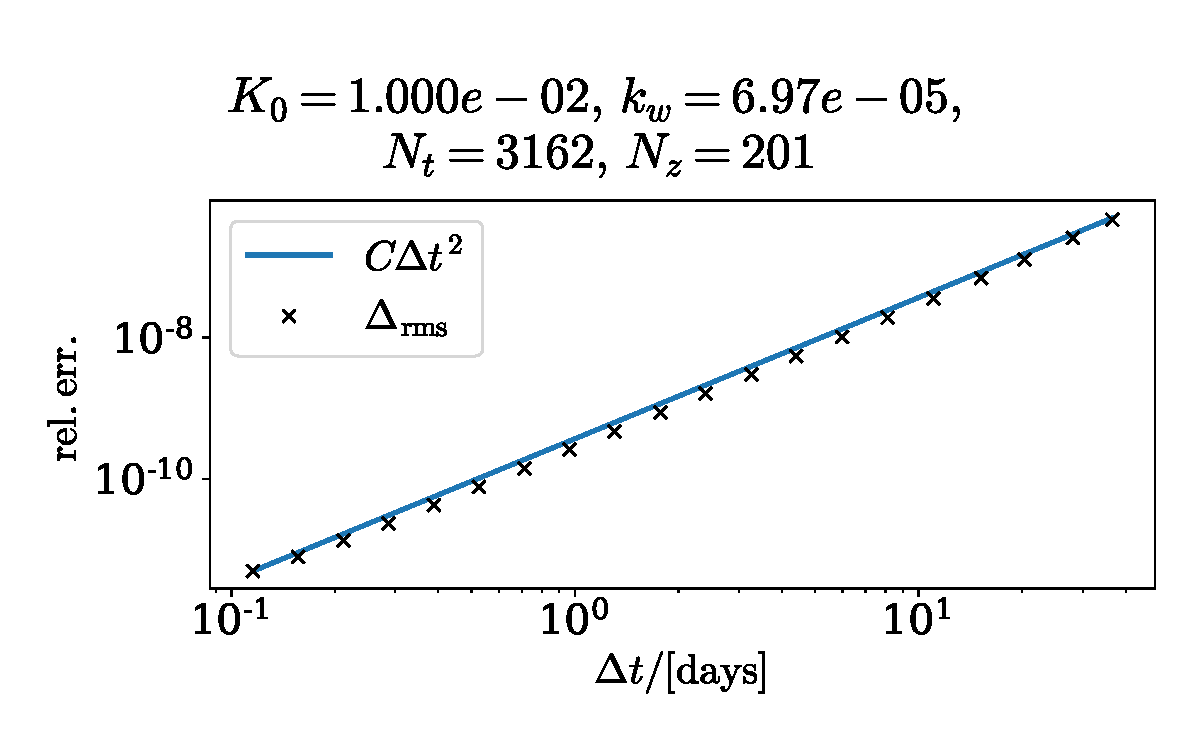
\includegraphics[width=.49\textwidth]{../plots/prob3_conv_test_t}
        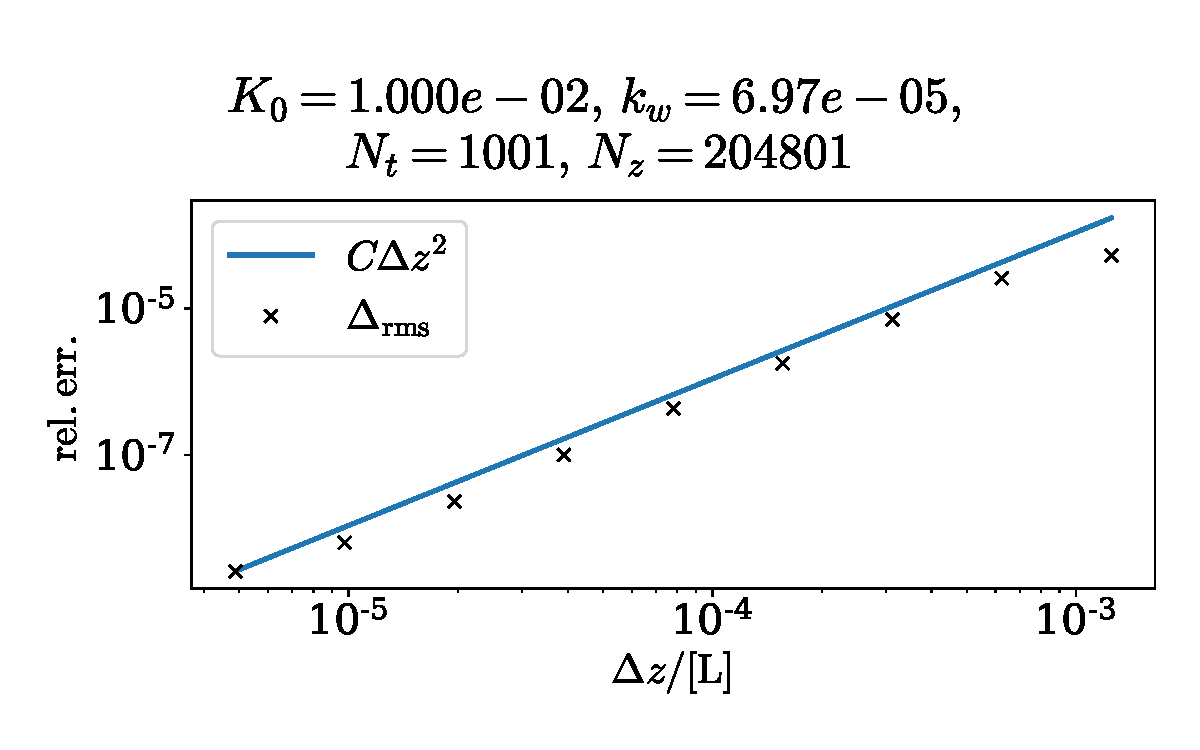
\includegraphics[width=.49\textwidth]{../plots/prob3_conv_test_z}
        \caption{Error, as a function of step length in both time and space.}
        \label{prob3 conv}
    \end{figure}

    \autoref{prob3} shows the concentration of \ce{CO2} as a function of time, as given by the simulation. The units of $C$ in this exercise is $\si{mol / m^{-3}}$, so the "mass" given by the formula $M = \int \dd z C(z)$ is mol per square meter of ocean. Using $0.36 \cdot 10^{15}\si{m^2}$ as the value of the surface area of the global oceans, and $\SI{24}{g / mol}$ as the molar weight of carbon in \ce{CO2}, the total wieght of the carbon stored in the ocean is plotted in \autoref{prob3 mass}. This simulation results in a uptake of $\Delta M = 504.8 \cdot 10^{15} \si{g}$ carbon over 10 years, i.e. an average absorption rate of $50.48 \cdot 10^{15} \si{g/year}$.

    \begin{figure}
        \centering
        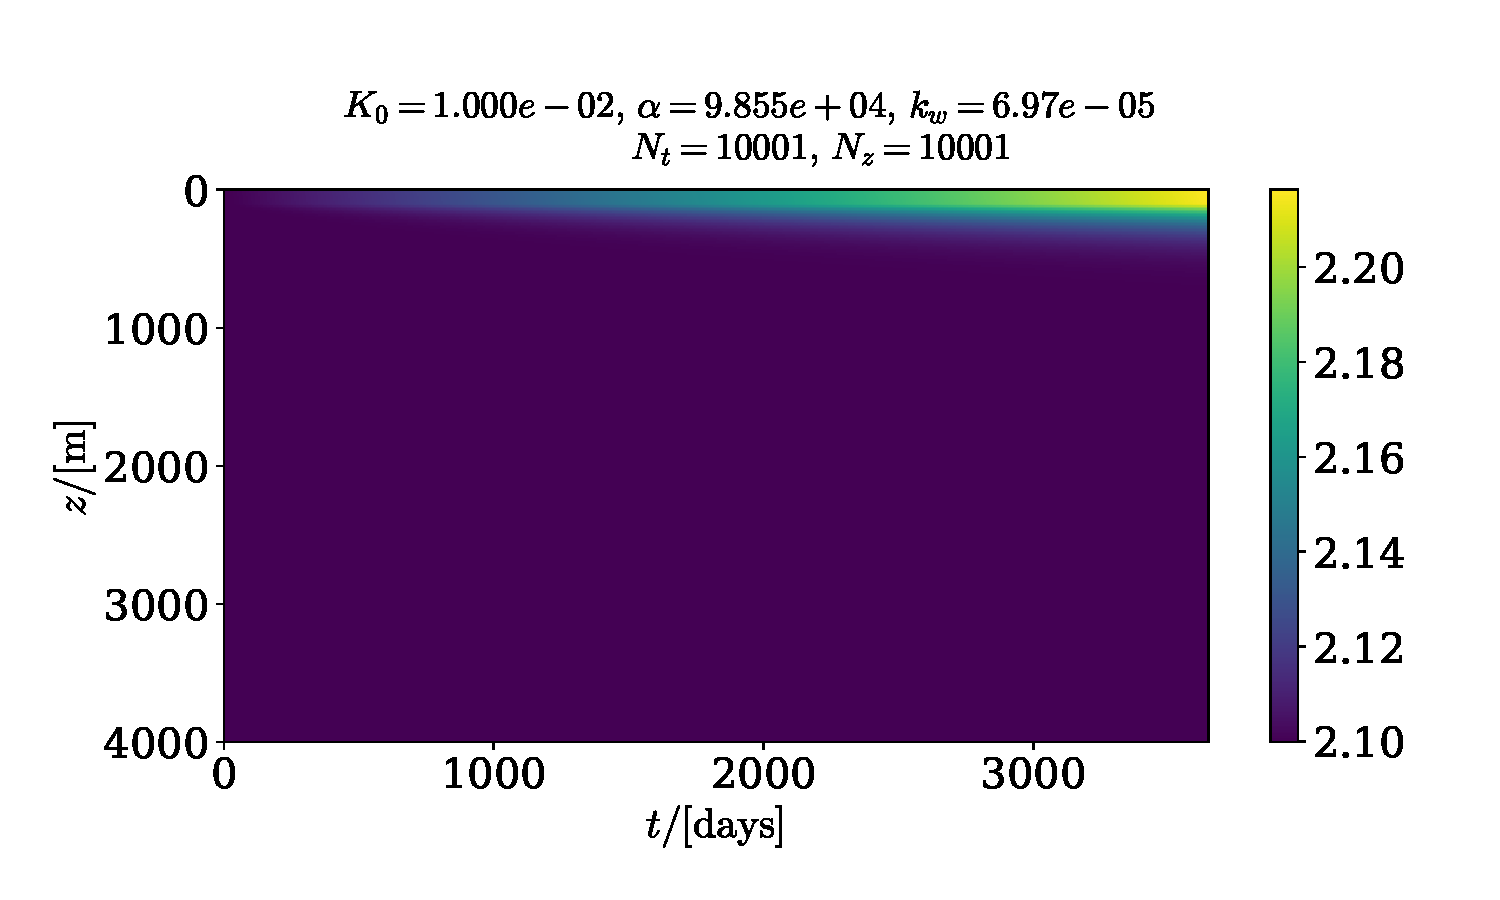
\includegraphics[width=.60\textwidth]{../plots/prob3}
        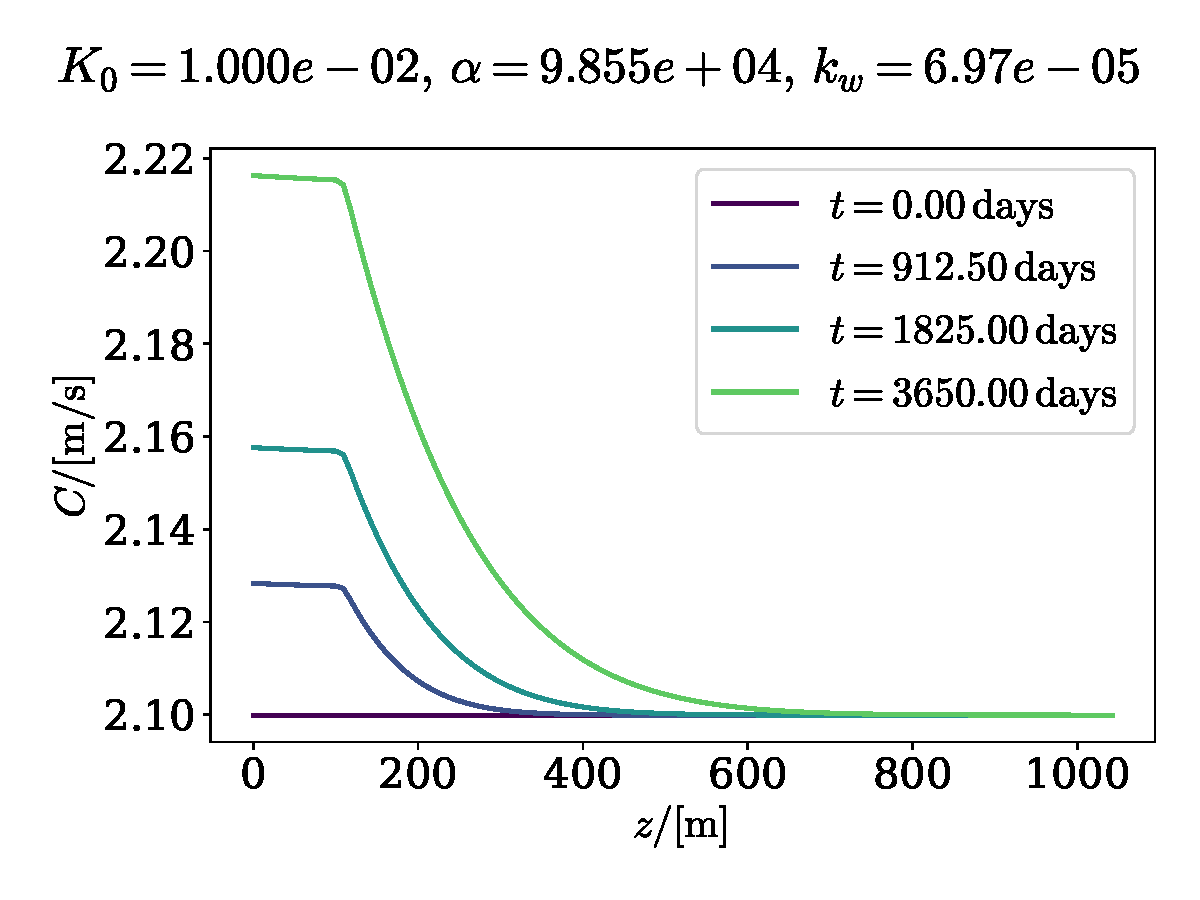
\includegraphics[width=.39\textwidth]{../plots/prob3_i}
        \caption{The concentration of \ce{CO2} in as a function of time, over 10 years.}
        \label{prob3}
    \end{figure}
    \begin{figure}
        \centering
        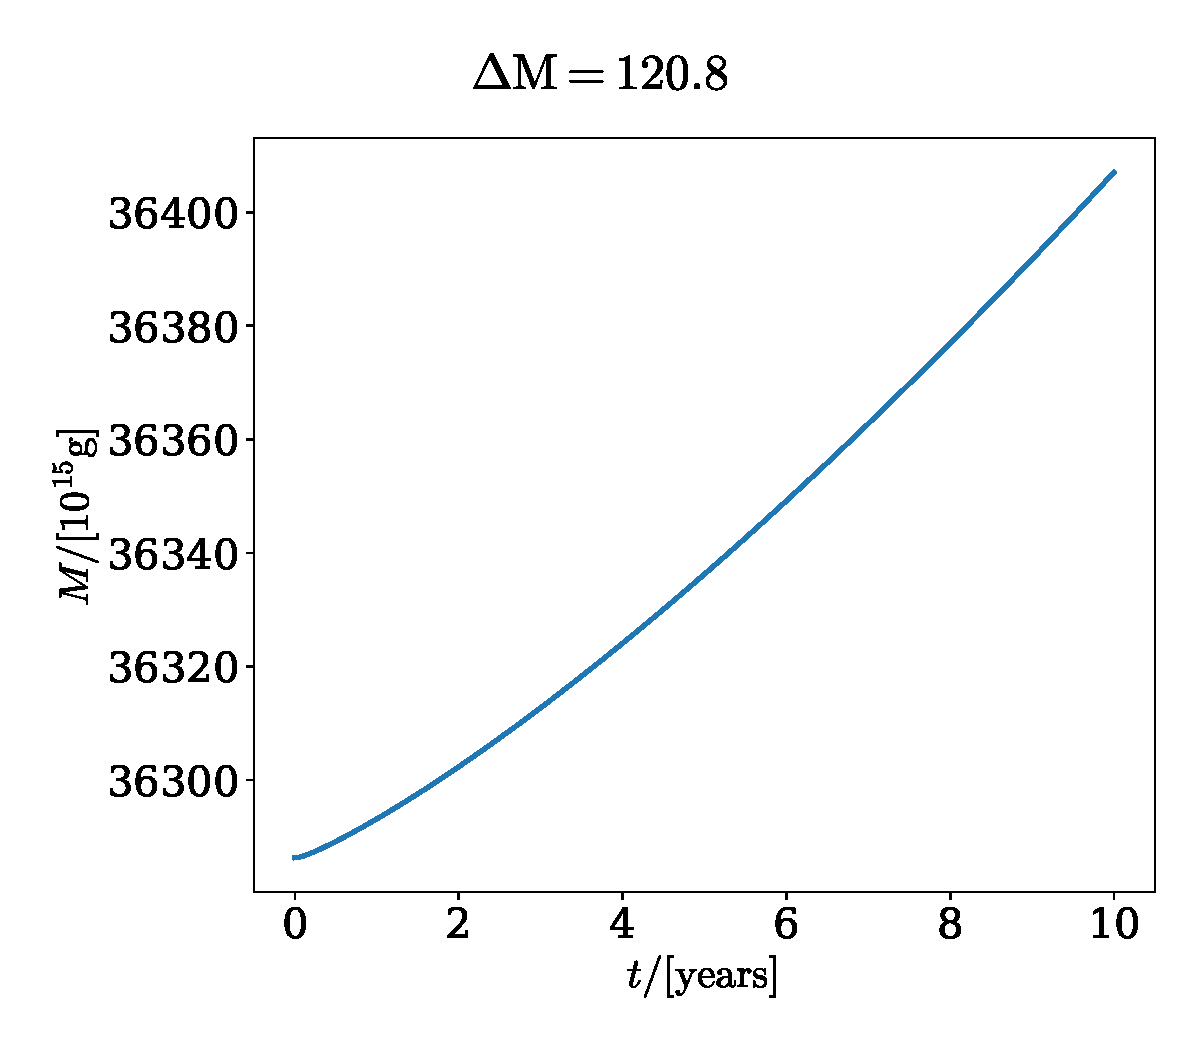
\includegraphics[width=.60\textwidth]{../plots/prob3_M}
        \caption{The concentration of \ce{CO2} in as a function of time, over 10 years.}
        \label{prob3 mass}
    \end{figure}


    \bibliography{report}
    \bibliographystyle{plain}   
\end{document}